% !TeX spellcheck = de_DE

\chapter{Methodologies}
\label{chap:k2}

The following sections introduce the principles of 3D lane marking reconstruction method of this work, based on the work flow shown in \cref{fig:FlowChart}.

\cref{sec:LineExtraction} describes the applied standard line detection algorithm for labeling the lane markings. 

To relate the object coordinates of a point with its image coordinates, \cref{sec:Geometry} introduces the imaging properties of aerial images and their mathematical models, including the collinearity equation and lens distortion correction.

\cref{sec:LineFitting} introduce the principle of line fitting and further presents the orthogonal regression model with line equations in two-point form. 

A non-linear LS model is derived and estimated in \cref{sec:LSadj} to elaborate the usage of line fitting with the combination of collinearity condition for 3D lane marking reconstruction.

In \cref{sec:LineProjectionOnDSM} the generation of approximate 3D line segments is described, as initial values of unknown quantities are required in nonlinear LS estimation.


\begin{figure}
	\centering
	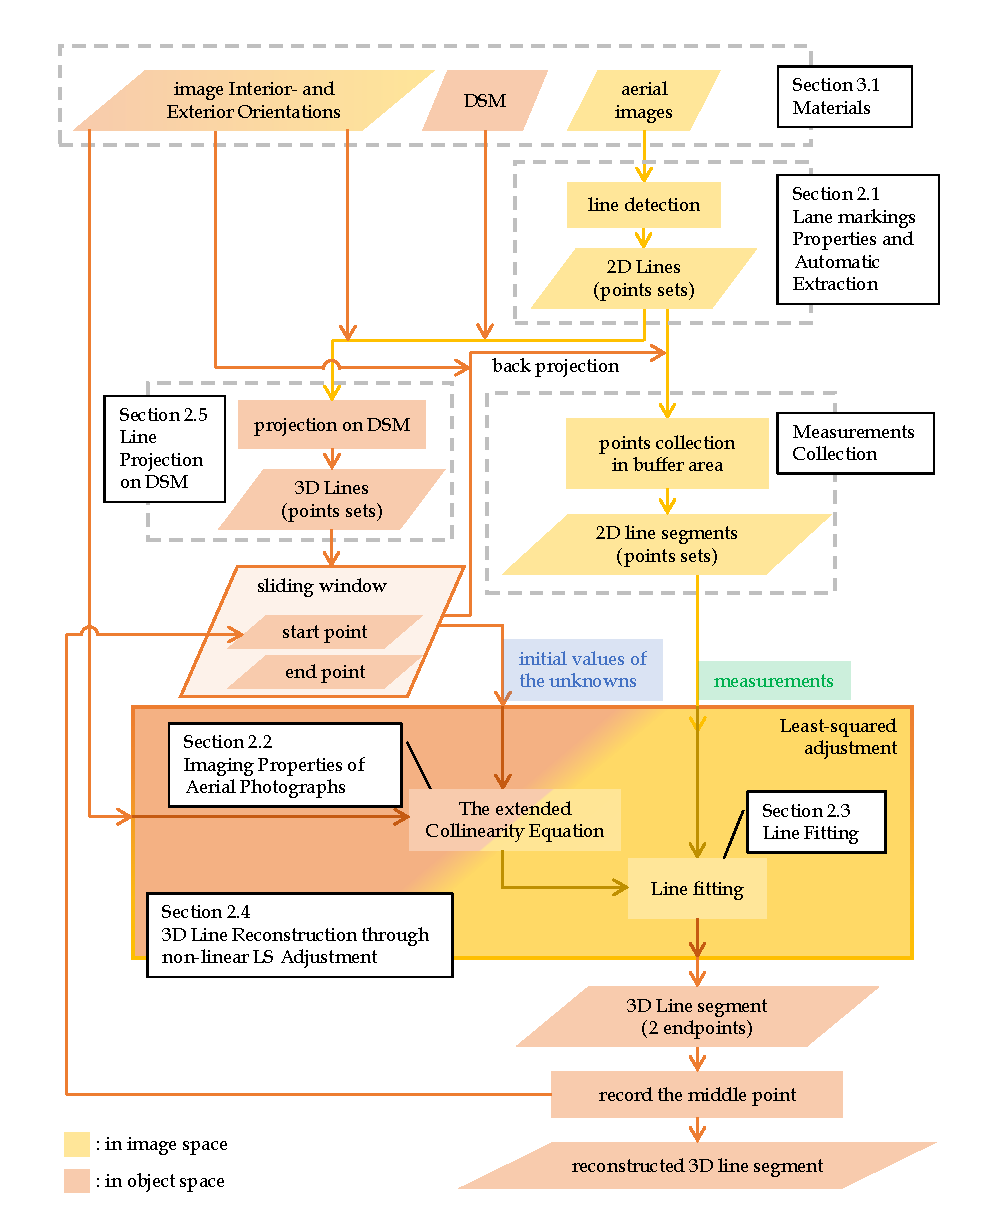
\includegraphics[width=\textwidth]{workflow.pdf}
	\caption{\small The work flow}
	\label{fig:FlowChart}
\end{figure}

\clearpage


%%%%%%%%%%%%%%%%%%%%%%%%%%%%%%%%%%%%%%%%%%%%%%%%%%%%%%%%
\section{Lane markings Properties and Automatic Extraction}
\label{sec:LineExtraction}

The appearance of lane markings on German roads including line type, color and width is specified depending on the road type. Different line types of lane markings are shown in \cref{fig:LaneMarkingTypes} and their line widths are defined in \cref{tab:LaneMarkingWidths}. As shown in \cref{tab:DashedLaneMarkingLengths}, the dashed lane markings on motorways have 6 meter length.

Because of the appearance, the problem of lane marking detection can be treated as a line detection problem. We restrict the proposed framework to lane markings with single white lines (dashed or continuous) of 0.3 meter width. Other types like in restricted zone, double lines, parking areas, temporal yellow lines in construction sites etc, are excluded.% https://www.transchool.lee.army.mil/adso/documents/zeichen.pdf


\begin{figure}
	\centering
	\subfloat[\small Continuous line]{\fbox{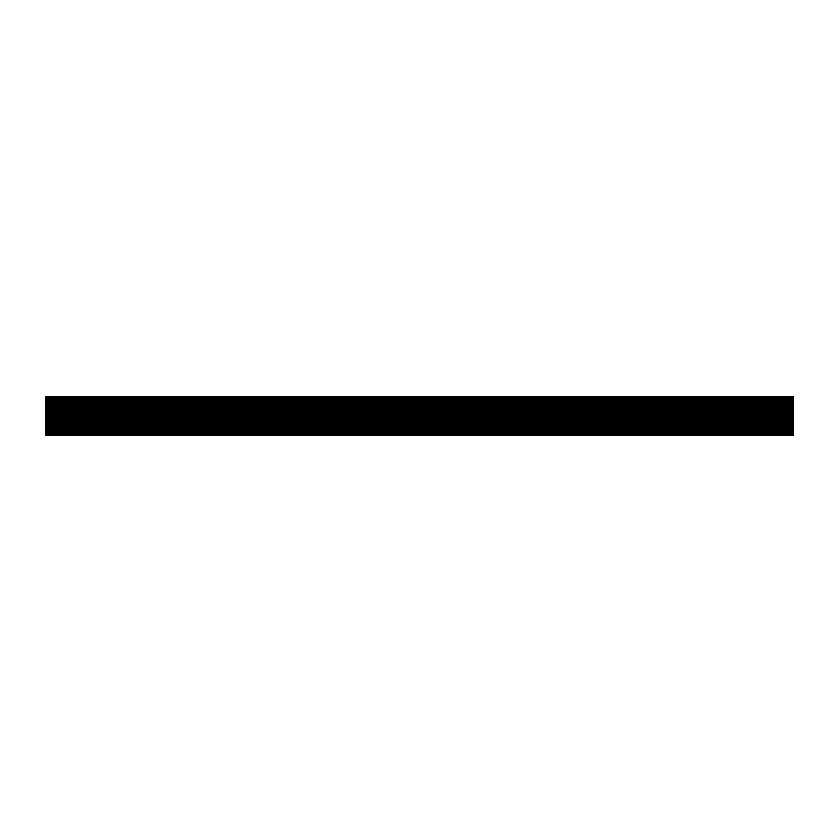
\includegraphics[width=0.3\textwidth, trim={0 150 0 150},clip=true]{Laengsmarkierung_durchgehend.pdf}}}
	\quad
	\subfloat[\small Dashed line]{\fbox{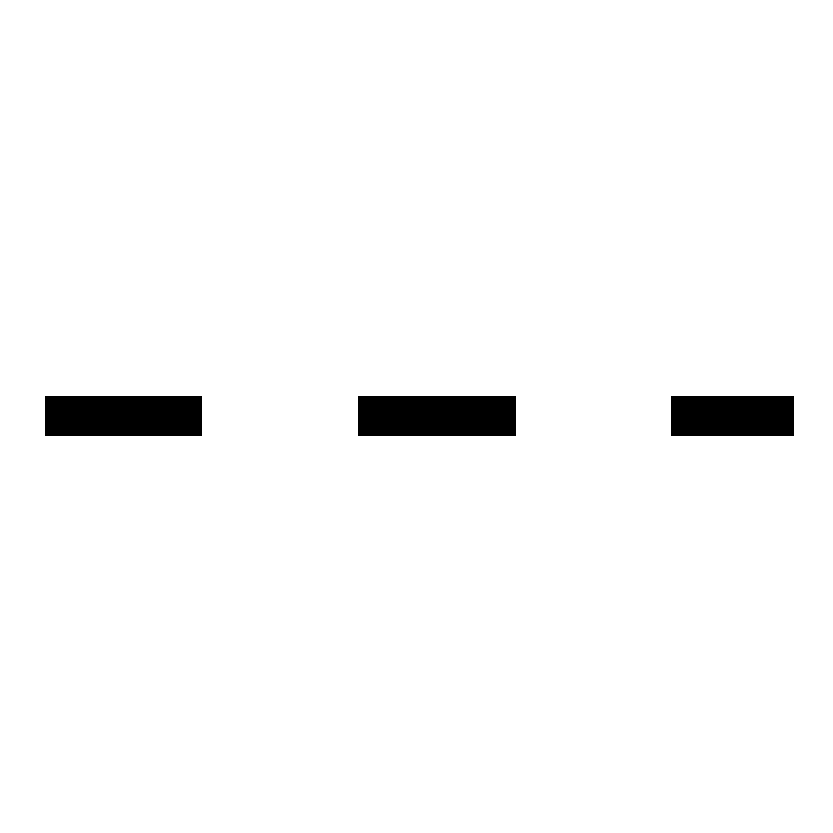
\includegraphics[width=0.3\textwidth, trim={0 150 0 150},clip=true]{Laengsmarkierung_unterbrochen.pdf}}}
	\newline
	\subfloat[\small Continuous and dashed double lines]{\fbox{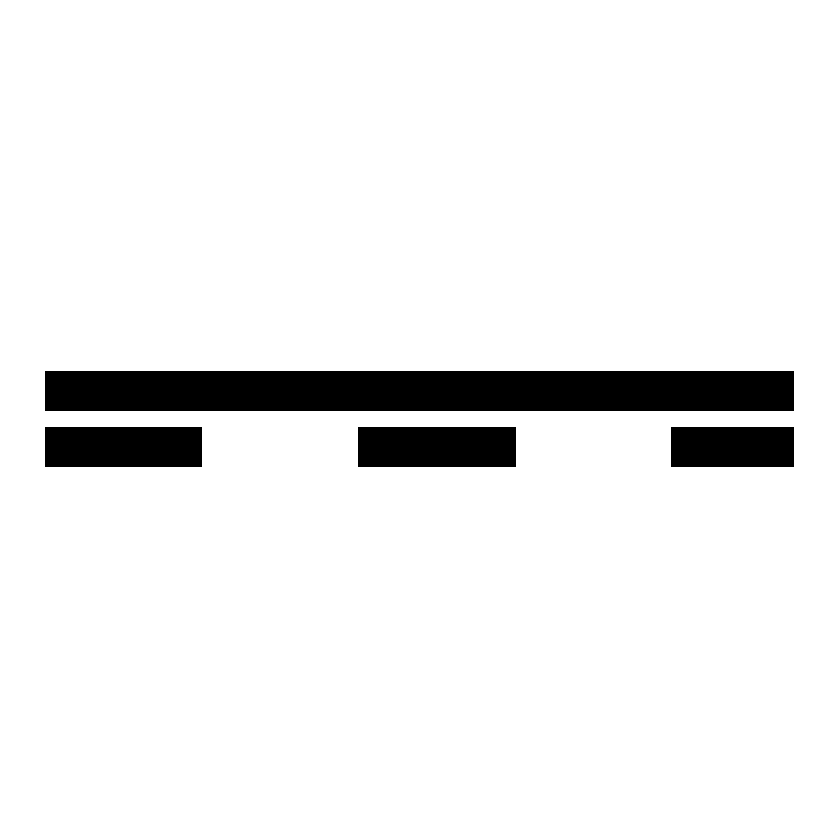
\includegraphics[width=0.3\textwidth, trim={0 150 0 150},clip=true]{Laengsmarkierung_unterbrochen_durchgehend.pdf}}}
	\quad
	\subfloat[\small Continuous double lines]{\fbox{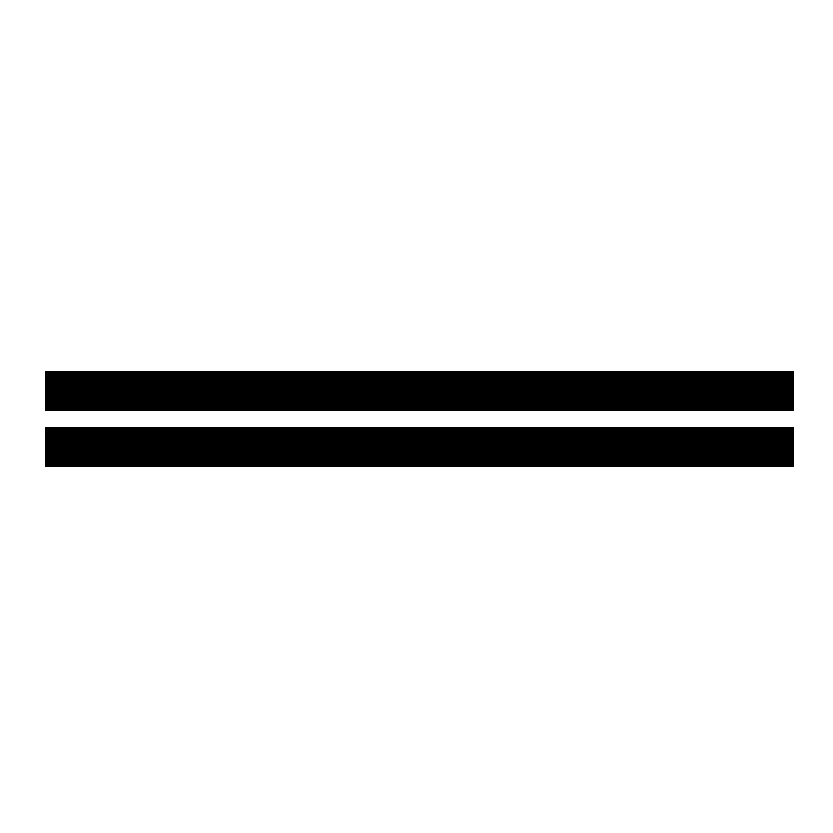
\includegraphics[width=0.3\textwidth, trim={0 150 0 150},clip=true]{Laengsmarkierung_durchgehend_doppelt.pdf}}}
	\quad
	\subfloat[\small Dashed double lines]{\fbox{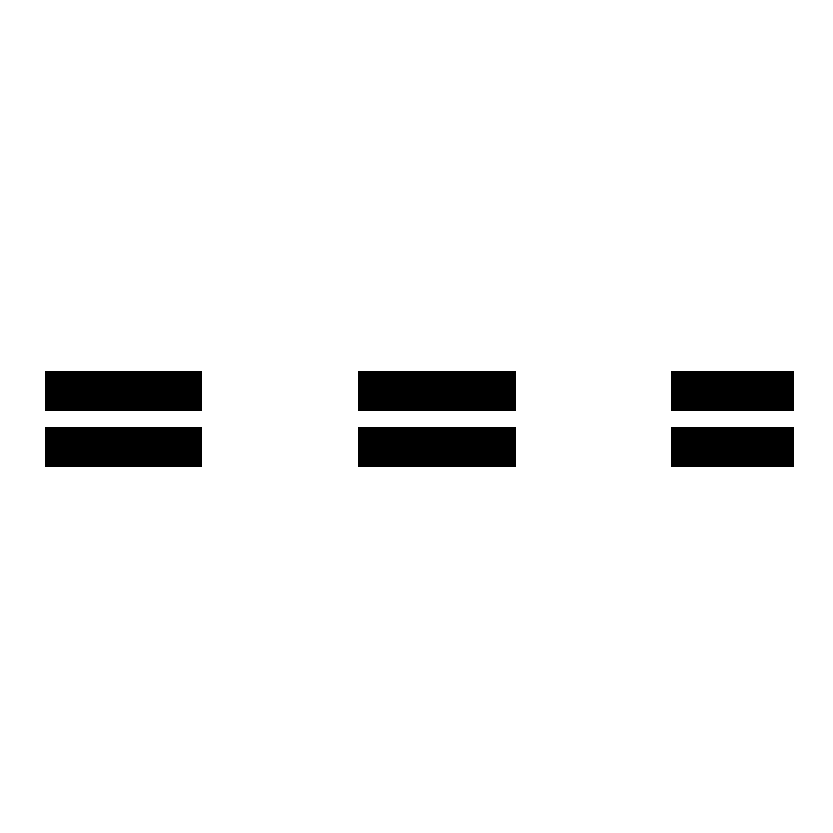
\includegraphics[width=0.3\textwidth, trim={0 150 0 150},clip=true]{Laengsmarkierung_unterbrochen_doppelt.pdf}}}
	\caption{\small Line types of lane markings \cite{RMS1}}
	\label{fig:LaneMarkingTypes}
\end{figure}

%\setlength{\floatsep}{16pt plus 1.0pt minus 2.0pt}
\begin{table} [h!]
	\centering
	\begin{tabular}{l|cc}
		\toprule
		& motorways\footnote{\label{motorway}and corresponding roads in the sense of the VwV-StVO to § 42 to mark 330 (motorway) II} & other roads\\
		\midrule
		narrow lines & $0.15$ [m] & $0.12$ [m] \\
		wide lines   & $0.30$ [m] & $0.25$ [m] \\
		\bottomrule
	\end{tabular}
	\caption{\small Widths of lane markings \cite{RMS1}}
	\label{tab:LaneMarkingWidths}
	% Der Deutsche Verkehrssicherheitsrat
	% https://www.dvr.de/download/publikationen-schriftenreihe-17.pdf
	% Richtlinien für die Markierung von Straßen (RMS) Teil 1
	
\end{table}

\setlength{\floatsep}{16pt plus 1.0pt minus 2.0pt}
\begin{table} [h!]
	\centering
	\begin{tabular}{l|ccc}
		\toprule
		& motorways\textsuperscript{\ref{motorway}} & \multicolumn{2}{c}{other roads}\\
		\cline{3-4}
		&           & in town & out of town\\
		\midrule
		line / gap  & $6$ [m] / $12$ [m] & $3$ [m] / $6$ [m] & $4$ [m] / $8$ [m]\\
		\bottomrule
	\end{tabular}
	\caption{\small Lengths of dashed lane markings with ratio 1:2 \cite{RMS1}}
	\label{tab:DashedLaneMarkingLengths}
	% Der Deutsche Verkehrssicherheitsrat
	% https://www.dvr.de/download/publikationen-schriftenreihe-17.pdf
	% Richtlinien für die Markierung von Straßen (RMS) Teil 1
\end{table}


\clearpage

% https://en.wikipedia.org/wiki/Edge_detection#Approaches
There are many algorithms for line detection. Prewitt line detector uses two orthogonal gradient operators, and the pixels in the operators are of same weights. Sobel detector also uses two orthogonal gradients operators, but the weights of pixel in operators are not equal ---the closer the pixel to the center of operator, the higher weight it has. Canny edge detector searches local extrema of gradient to locate the positions of line features and is still a state-of-the-art edge detector. Edge-detectors that perform better than the Canny usually require higher computational complexities or a greater number of parameters. Edge drawing \cite{Topal2012} first spots anchors along rows and columns by Sobel detector, and then joins these anchors to extract line features.

In this work, the principle to extract line features is to firstly derive the line direction for each pixel by using partial derivatives of a Gaussian smoothing kernel. Pixels that have a local maximum in the second directional derivative perpendicular to the line direction are marked as line points. By thresholding their second directional derivative values, the accepted line points are then linked and connected.\cite{Steger1998}

The resulting connected points which compose a line are of sub-pixel precision. \cref{fig:LineExtraction} shows the extracted lines on part of the masked original image.
% http://www.mvtec.com/doc/halcon/11/en/lines_gauss.html

\begin{figure}
  \centering
  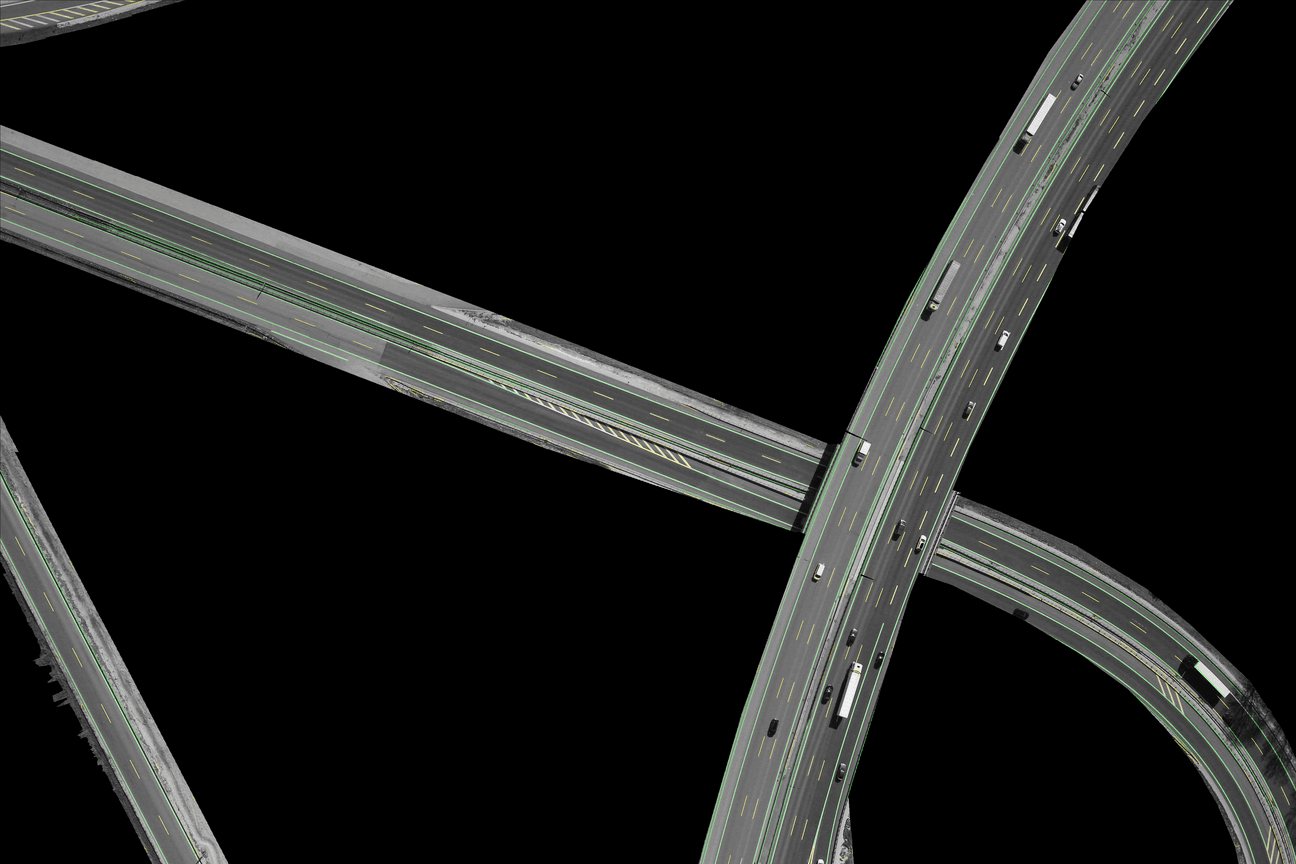
\includegraphics[width=0.9\textwidth, trim=750 260 200 360,clip]{ML1234_extlines_rsz.png}
  \caption{\small Lane markings Extraction. The extracted long lane-lines are marked in green and the dashed ones are in yellow.  Note that both cases are reconstructed into 3D with the same framework; different colors here are only for illustration.}
  \label{fig:LineExtraction}
\end{figure}


\clearpage
%%%%%%%%%%%%%%%%%%%%%%%%%%%%%%%%%%%%%%%%%%%%%%%%%%%%%%%%
\section{Imaging Properties of Aerial Photographs}
\label{sec:Geometry}

This section describes the geometric model of the projection of 3D points into the image generated by a real camera. We first restrict the discussion in \cref{subsec:Collinearity} to central perspective projection where the collinearity equation originates from. We then model deviations from this model, addressing real cameras with imperfect lenses, in \cref{subsec:LensDistortion}.

\subsection{Collinearity Equations}
\label{subsec:Collinearity}
We assume frame photography, i.e. photographs exposed on a frame chip in one instant, and assume the central projection model with cameras that have a single viewpoint and a planar sensor and being straight line-preserving. Collinearity indicates the condition that the image point (on the sensor plate of the camera), the observed point (in object space) and the projection center of the camera were aligned at the moment the picture was taken. Every measured point leads to two collinearity equations, describing transformations from object space to image coordinates:
\begin{equation} \label{eq:collinearity}
\begin{split}
x = x_0 -c \dfrac {r_{11}(X-X_0) + r_{21}(Y-Y_0) + r_{31}(Z-Z_0)} {r_{13}(X-X_0) + r_{23}(Y-Y_0) + r_{33}(Z-Z_0)} \\
y = y_0 -c \dfrac {r_{12}(X-X_0) + r_{22}(Y-Y_0) + r_{32}(Z-Z_0)} {r_{13}(X-X_0) + r_{23}(Y-Y_0) + r_{33}(Z-Z_0)}
\end{split}
\end{equation}
where\newline
$(x, y)$: image coordinates of the point \newline
$(x_0, y_0)$: image coordinates of principal point \newline
$c$: principal distance; focal length \newline
$(X, Y, Z)$: object coordinates of the point \newline
$(X_0, Y_0, Z_0)$: object coordinates of projection center \newline
$r_{11},...,r_{33}$: elements of the rotation matrix R (orthogonal 3$\times$3-matrix from object space to image space, with 3 independent angles $\omega$, $\phi$ and $\kappa$)

\subsection{Lens Distortion Correction}
\label{subsec:LensDistortion}

An original image has some degree of deviations from perspective mapping due to lens distortion, lens refraction or non-planarity of the sensor surface. There are several models to describe these perturbing effects and can be used to undistort the images, resulting in rectified images which are now straight line-preserving.
 
A subset of physical distortion model \cite{Fraser1997} is chosen, with two radial symmetric distortion parameters $A_1$ and $A_2$, two asymmetric parameters $B_1$ and $B_2$, and a scaling $C1$ and an affine shearing parameter $C_2$. Assuming $x$ and $y$ to be the distorted image coordinates, the corrections $\Delta x$ and $\Delta y$ are then calculated by the following equations:
\begin{equation} \label{eq:LensDistortion}
\begin{split}
\Delta x &= x_p + A_1x_*(r^2-R_0^2) + A_2x_*(r^4-R_0^4) + B_1(r^2+2x_*^2) + B_22x_*y+C_2y \\
\Delta y &= y_p + A_1y  (r^2-R_0^2) + A_2y  (r^4-R_0^4) + B_1(r^2+2y^2)   + B_22x_*y
\end{split}
\end{equation}
with $r=\sqrt{x_*^2+y^2}$, $x_*=\dfrac{x}{C_1}$ and radius\footnote{At the radius $R_0$ the radial symmetric distortion is zero by definition, which avoids too high distortion values at the edges and reduces the correlation with the focal length.} $R_0$ being set %to 0.014m which corresponds 
to a third of the sensor diagonal.

The undistorted image coordinates $x\prime$ and $y\prime$ are then calculated by
\begin{equation} \label{eq:undistortedimgcoord}
\begin{split}
x\prime=x+\Delta x \\
y\prime=y+\Delta y
\end{split}
\end{equation}

\subsection{Extended Collinearity Equation}
\label{subsec:ExtendedCollinearity}
As real cameras only approximate the perspective camera model, lens distortion correction can be additionally included in the collinearity model, attempting to correct the pixel positions so that they obey the perspective model with sufficient accuracy.%[W. Förstner et al. 2016] % The reference is not the original one

By inserting \eqref{eq:collinearity} and \eqref{eq:LensDistortion} into \eqref{eq:undistortedimgcoord} , the relationship between a 3D point $\mathbf{P}(X, Y, Z)$ and its corresponding distorted image coordinates $\mathbf{p}(x,y)$ can be described as
\begin{equation} \label{eq:expandedcollinearity}
\begin{split}
x =& x_0-c\dfrac{r_{11}(X-X_0)+r_{21}(Y-Y_0)+r_{31}(Z-Z_0)}{r_{13}(X-X_0)+r_{23}(Y-Y_0)+r_{33}(Z-Z_0)} \\
&-(x_p + A_1x_*(r^2-R_0^2) + A_2x_*(r^4-R_0^4) + B_1(r^2+2x_*^2) + B_22x_*y+C_2y)\\
y =& y_0-c\dfrac{r_{12}(X-X_0)+r_{22}(Y-Y_0)+r_{32}(Z-Z_0)}{r_{13}(X-X_0)+r_{23}(Y-Y_0)+r_{33}(Z-Z_0)} \\
&-(y_p + A_1y  (r^2-R_0^2) + A_2y  (r^4-R_0^4) + B_1(r^2+2y^2)   + B_22x_*y)
\end{split}
\end{equation}

To express \eqref{eq:expandedcollinearity} shortly, a function $\mathcal{G}$ is defined as
\begin{equation} \label{eq:Gfunction}
\mathbf{p} = \mathcal{G}(\mathbf{q},\mathbf{P}) 
\end{equation}

which takes the interior and exterior orientations as well as the lens distortion parameters of a camera $\mathbf{q}(x_0,y_0,c,X_0,Y_0,Z_0,r_{11},...,r_{33},A_1,A_2,B_1,B_2,C_1,C_2)$ and the position of a 3D point $\mathbf{P}(X, Y, Z)$, and returns the corresponding distorted image coordinates $\mathbf{p}(x,y)$.

\clearpage
%%%%%%%%%%%%%%%%%%%%%%%%%%%%%%%%%%%%%%%%%%%%%%%%%%%%%%%%
\section{Line Fitting}
\label{sec:LineFitting}

Line fitting is the process of constructing an infinite straight line that has a best fit to a 2D dataset. One of the approaches is linear regression which attempts to find the linear function that "best" predicts the dependent variable values as a function of the independent variable. In this work, "best" predict will be understood as in the \gls{ls} approach: minimization of the sum of squared residuals (differences between the measured and the estimated values of the dependent variable).

In the case of standard linear regression, the regressor $x$ is assumed error free, inconsistencies\footnote{The word "inconsistencies" indicates the unobserved random errors, also called as measurement errors.} are only for the dependent variable $y$. Geometrically it means that the vertical distances from observed data to the fitted line is minimized. To minimize the perpendicular distances from the data points to the regression line, a orthogonal regression model is derived in \cref{subsec:OrthogonalRegression}.

For a later combination with point-wise extended collinearity equation \eqref{eq:Gfunction} in next section, the aim is to fit the line equation in two-point form to the observed dataset. For such nonlinear functional relation between variales, a nonlinear LS model is derived in \cref{subsec:NonLinear}.

A functional model is unsolvable when the assumed "dependent" variable is indeed not a function of the independent variables, i.e. the assumed functional relation does not really exist. Take an observed set of 2D points with their Cartesian coordinates $\{x_i,y_i\}^n_{i=1}$ on a vertical line $x=constant$ for example. Their $y$ values have no dependency on their $x$ values, i.e. knowledge of $x$ tells nothing about $y$. Therefore, for this dataset, the functional model $y=f(x)$ is singular. In such cases, however, $x$ is a function of $y$ (which is actually a constant function) and the equation system which models the dependent variable $x$ being a function of the independent variable $y$ becomes solvable. Regarding the dataset used in this work (which will be described with more details in \cref{sec:Materials}) where the observed 2D points scatter mainly in column direction in image space, the functional relation between variables $x$ and $y$ will be setup as $x=f(y)$ to avoid weakly solvable equations system.

%\subsection{Simple Linear Regression}
%\label{subsec:LinearRegression}

%A simple linear regression model describes the linear relationship between a dependent variable and a regressors (an independent variable). By assuming the regressor $y$ being exactly measured without errors, it accounts only for errors $e_x$ in the dependent variable $x$.

%Given a dataset $\{x_i,y_i\}^n_{i=1}$ of $n$ points on a 2D plane, the model takes the form:
%\begin{equation} \label{eq:SimpleLinearRegression}
%x_i - e_{x_i} = a_0 + a_1y_i
%\end{equation}
%where the regression coefficients $a_0$ and $a_1$ are the unknown parameters to be estimated; the error variable $e_x$ is an unobserved random variable that adds noise to the linear relationship between the dependent variable $x$ and regressor $y$.
%https://en.wikipedia.org/wiki/Linear_regression#Assumptions


\subsection{Orthogonal Regression}
\label{subsec:OrthogonalRegression}
A linear regression model describes a dependent variable as a linear function of the regressor (an independent variable). Given a dataset $\{x_i,y_i\}^n_{i=1}$ of $n$ points on a 2D plane, in the case when both dependent variable $x_i$ and regressor $y_i$ are measured with errors, a linear regression model takes the form:
\begin{equation} \label{eq:MixModel1-1}
x_i - e_{x_i} = %a_0 + a_1(y_i-e_{y_i}) = 
a_0 + a_1\bar{y_i}
\end{equation}
where the regression coefficients $a_0$ and $a_1$ are the unknown parameters to be estimated, $\bar{y_i}$ denotes the true but unobserved regressor, and the error variable $e_{x_i}$ is an unobserved random variable that adds noise to the linear relationship between the dependent variable $x$ and true regressor $\bar{y_i}$. Whereas the true regressor $\bar{y_i}$ is observed with an error $e_{y_i}$ in the pseudo observation equation:
\begin{equation} \label{eq:MixModel1-2}
y_i-e_{y_i} = \bar{y_i}
\end{equation}
Such models, as the combination of \eqref{eq:MixModel1-1} and \eqref{eq:MixModel1-2}, that take into account the measurement errors of both dependent variables and regressors, are errors-in-variables models. Further more, for the case of equal error variances, i.e. when $\delta=\dfrac{\sigma_{e_x}}{\sigma_{e_y}}=1$, it is a orthogonal regression model which minimizes the perpendicular distances from the data points to the regression line.

\subsection{Orthogonal Regression in Two-point Form}
\label{subsec:NonLinear}

The two-point form of a infinite line in the Cartesian plane passing through the points $(x_1,y_1)$ and $(x_2,y_2)$ is given by:
\begin{equation} \label{eq:LineInTwoPointForm}
(x-x_1) = \dfrac{(x_2-x_1)}{(y_2-y_1)}\times y-y_1
\end{equation}
with $y_2\neq y_1$, where $(x,y)$ is any point on the line.

Let the unknown coordinates of two different points on a line in 2D space be $(x_1,y_1)$ and $(x_2,y_2)$ and the observed 2D points be $\{x_i,y_i\}^n_{i=1}$ with measurement errors $e_{x_i}$ and $e_{y_i}$ in both variables. The orthogonal regression model in two-point form is: 
\begin{equation} \label{eq:MixModel2-1}
x_i - e_{x_i}= (x_1-\dfrac{(x_2-x_1)}{(y_2-y_1)}\times y_1) + \dfrac{(x_2-x_1)}{(y_2-y_1)}\times \bar{y_i}
\end{equation}
\begin{equation} \tag{\ref{eq:MixModel1-2} revisited}
y_i-e_{y_i} = \bar{y_i}
\end{equation}

To express \eqref{eq:MixModel2-1} and \eqref{eq:MixModel1-2} shortly, a function $\mathcal{F}$ is defined as

\begin{equation} \label{eq:Ffunction}
\hat{\mathbf{p}} = \mathcal{F}(\mathbf{p}_s,\mathbf{p}_e,y)
\end{equation}

which takes 2D coordinates of a start-point $\mathbf{p_s}(x_s,y_s)$ and an end-point $\mathbf{p_e}(x_e,y_e)$ that define an infinite line, and takes the measured y-coordinate $y$ of an image point $\mathbf{p}(x,y)$, and returns the estimated image coordinates $\mathbf{\hat{p}}(\hat{x},\hat{y})$ which lies on the infinite line $\overline{\mathbf{p_s}\mathbf{p_s}}$.

Note that as a combination of \eqref{eq:MixModel2-1} and \eqref{eq:MixModel1-2}, function $\mathcal{F}$ is actually composed of
\begin{equation} \label{eq:Ffunction_xy}
\begin{split}
\hat{x} = \mathcal{F}^x(\mathbf{p}_s,\mathbf{p}_e,y)\\
\hat{y} = \mathcal{F}^y(\mathbf{p}_s,\mathbf{p}_e,y)
\end{split}
\end{equation}

\clearpage
%%%%%%%%%%%%%%%%%%%%%%%%%%%%%%%%%%%%%%%%%%%%%%%%%%%%%%%%
\section{3D Line Reconstruction with Nonlinear LS Adjustment}
\label{sec:LSadj}

In this section, the process of refining the position of a 3D line segment in the object space so that its back-projection in each image has a best-fit to the extracted line in the image space is described, as illustrated in \cref{fig:mainidea}.

\begin{figure}
	\centering
	\subfloat[Before optimization]{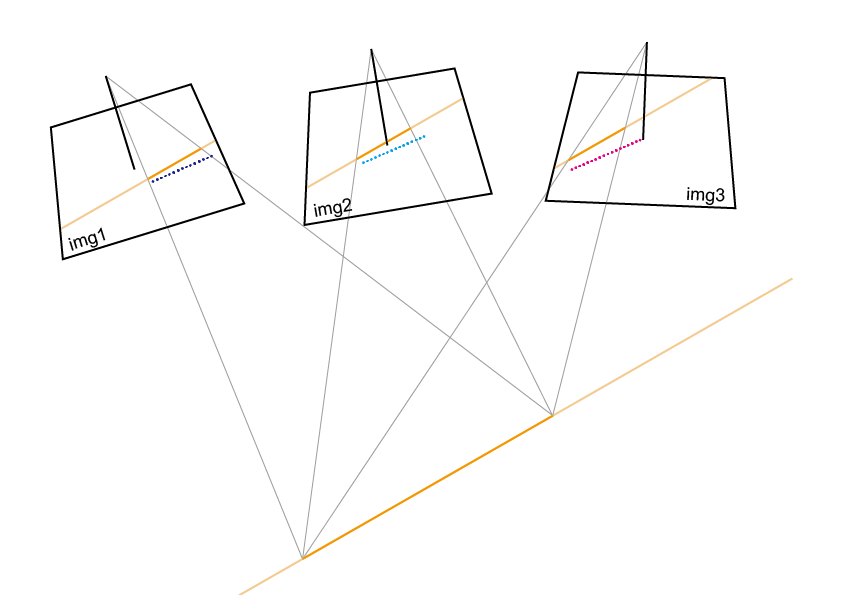
\includegraphics[width=0.9\textwidth]{2-4_1_1.png} \label{fig:beforeoptimization}}
	
	\subfloat[After optimization]{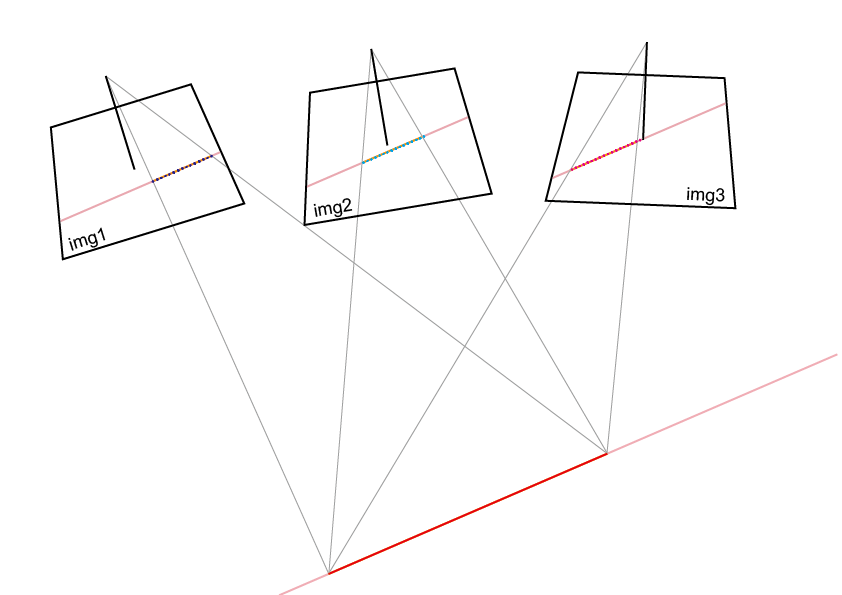
\includegraphics[width=0.9\textwidth]{2-4_1_2.png} \label{fig:afteroptimization}}
	\caption{\small Before reconstruction, the back projection of initial approximate 3D line segment does not best-fit the extracted 2D lines in the covering images. After optimization, the back-projection of the reconstructed line segment should be best fitting the extracted 2D lines in all the covering images.}
	\label{fig:mainidea}
\end{figure}


%%%%%%%%%%%%%%%%%% introduce the subsections
\cref{subsec:LSmodel} introduces the non-linear LS adjustment model with constraints. The observation equations for LS adjustment are set up in \cref{subsec:ObsEqua}. They describe the fitting of a straight line to the measurements, which are the extracted lines, in all covering images, where the fitting lines on different images are transformed from a single 3D straight line segment through the extended collinearity equation \eqref{eq:expandedcollinearity}. Regarding the fact that the collinearity is a point-wise condition, a line segment is represented by its two endpoints. Correspondingly, the observation equations in the LS model are line equations in two-point form. 

By satisfying the collinearity condition, single fitting line on an image spans a plane in $\mathbb{R}^3$. The corresponding lines from different views span several planes in $\mathbb{R}^3$, which are non-parallel to each other and should intersect in a line in $\mathbb{R}^3$. As this infinite line is the solution space of the LS estimation, at least two constraints on the location of the two endpoints of the targeted 3D line segment are necessary to avoid their arbitrary locations on this infinite line in $\mathbb{R}^3$. The constraint equations are modeled in \cref{subsec:ConEqua}.

So far the non-linear LS model has been setup. In \cref{subsec:LSadj} it is further linearized and the substitute linear LS model is estimated.

%\vspace{20pt}

%%%%% introduce the sliding window
To simplify the problem, a long lane-marking segment is partially reconstructed through a sliding window in the object space. Each segment is approximated by a straight line, taking into account the maximum curvature of the highway. 

In each sliding window, a segment is reconstructed, i.e. a complete non-linear LS adjustment is performed. Only the middle point of the reconstructed line segment is recorded. The sliding window then moves a stepsize forward, and the process of 3D reconstruction is performed again starting from the recorded middle point of the previous line segment. Another line segment is then reconstructed, with its middle point being recorded, and so on. These recorded middle points are in the end the nodes of the reconstructed line. This process is illustrated in \cref{fig:slidingwindow}.


\begin{figure}
	\centering
	\subfloat[The first line segment of "sliding window length" is reconstructed, with its starting point and its middle point of "step size" from the starting point being recorded.]{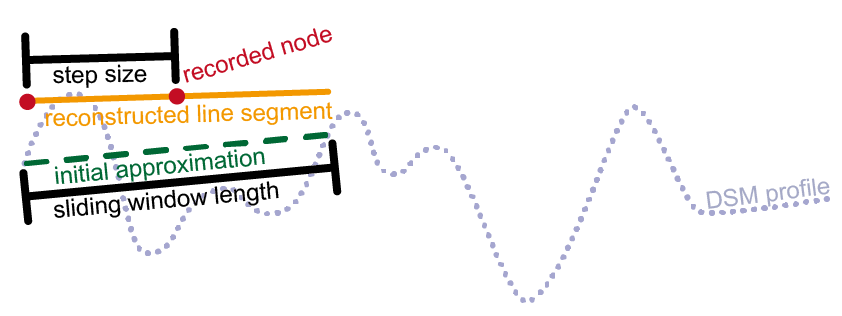
\includegraphics[width=0.9\textwidth]{2-4_2_1.png} \label{fig:slidingwindow1}}
	
	\subfloat[Starting from the recorded node of last process, another line segment of "sliding window length" will be reconstructed. i.e. the sliding window has moved "step size" forward.]{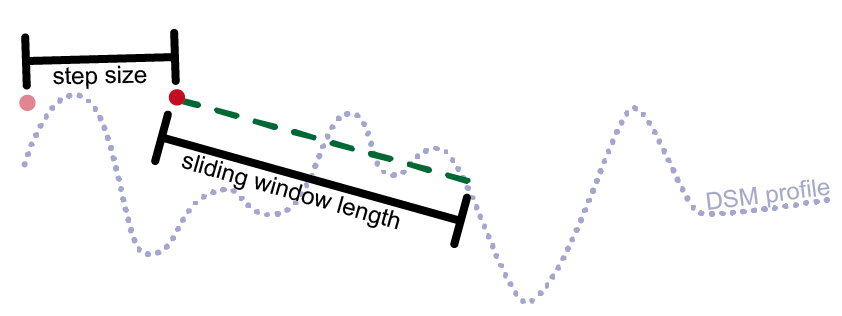
\includegraphics[width=0.9\textwidth]{2-4_2_2.png} \label{fig:slidingwindow2}}
	
	\subfloat[The point of "step size" length from the starting point on the reconstructed segment is recorded.]{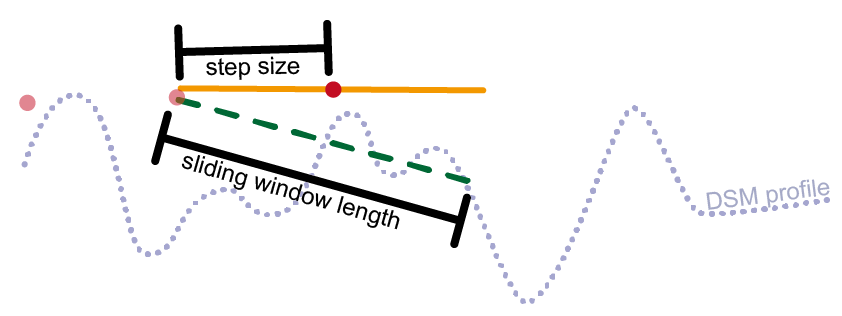
\includegraphics[width=0.9\textwidth]{2-4_2_3.png} \label{fig:slidingwindow3}}
	
	\caption{\small 3D reconstruction of a lane marking by a sliding window.}
	\label{fig:slidingwindow}
\end{figure}


%%%%% describe the collection of measurements 
The measurements for each reconstruction process are collected correspondingly, as shown in \cref{fig:measurementscollection} ---by back-projecting the initial line segment into image space and buffering 10 pixels width on each side. By this, all the extracted 2D line segments in this region are collected. As shown in \cref{fig:overlappingregion}, the reconsideration in overlapping region of successive sliding windows makes the reconstruction more robust.

\begin{figure}
	\centering
	\subfloat[The pink points represent all the extracted lines (in the form of sets of points). The green points are the endpoints of the back projected initial approximate 3D line segment.]{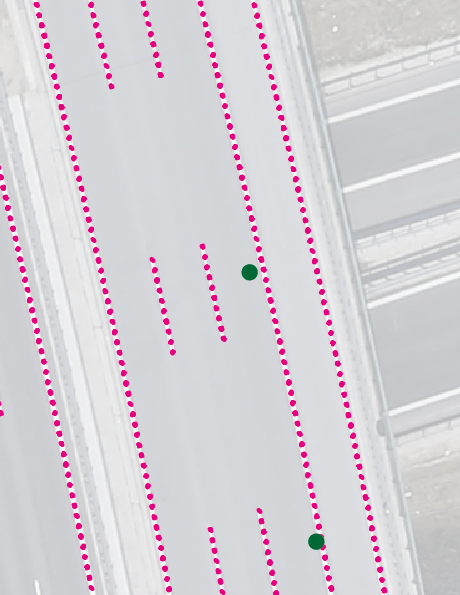
\includegraphics[width=0.45\textwidth]{2-4_3_1.png} \label{fig:measurementscollection1}}
	\subfloat[The points in the buffering area are collected as the measurements for LS adjustment.]{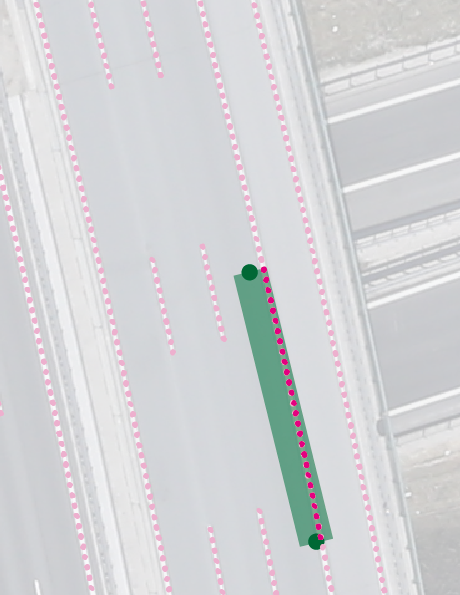
\includegraphics[width=0.45\textwidth]{2-4_3_2.png} \label{fig:measurementscollection2}}
	
	\caption{\small Measurements collection in image space.}
	\label{fig:measurementscollection}
\end{figure}


\begin{figure}
	\centering
	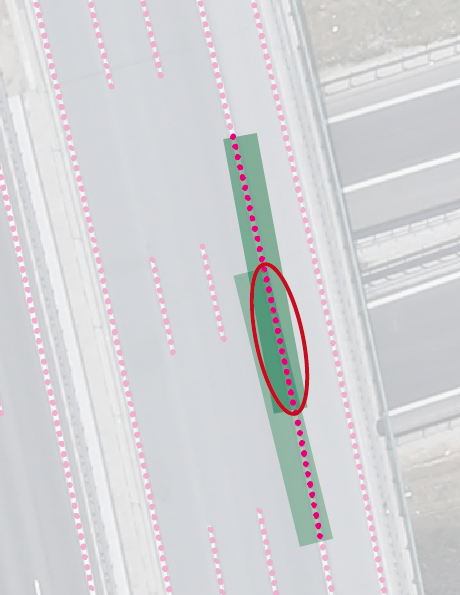
\includegraphics[width=0.45\textwidth]{2-4_3_3.png}
	\caption{\small The red circle points out the reconsidered measurements in successive sliding windows.}
	\label{fig:overlappingregion}
\end{figure}

\clearpage
\subsection{The Gauss-Markov Model with Constraints}
\label{subsec:LSmodel}

Adjustment theory deals with the optimal combination of redundant measurements/observations, together with the estimation of unknown parameters \cite{Teunissen2000}.

Given are the $N$ observations $\boldsymbol l=[l_n],\,n=1,2,...,N$, from which the $U$ unknown parameters $\boldsymbol x=[x_u],\,u=1,2,...,U$ are to be determined, with generally $U\leq N$.%, and the fixed $H$ constraints $\boldsymbol c_h=[h_h],\,h=1,2,...,H$

The Gauss-Markov model with $N$ nonlinear functions $\boldsymbol f(\boldsymbol x)=[f_n(\boldsymbol x)],\,u=1,2,...,U$ and the $H$ nonlinear constraints $\boldsymbol h(\boldsymbol x)=[h_\eta(\boldsymbol x)],\,\eta=1,2,...,H$ % !!!!!!!!!!!!$\boldsymbol c=[c_h],\,h=1,2,...,H$
($H<U$) between the unknowns can be written as:
\begin{equation} \label{eq:GM-ObsEq}
\boldsymbol l+\widehat{\boldsymbol v}=\boldsymbol f(\widehat{\boldsymbol x})\quad \textnormal{or}\quad \widehat{\boldsymbol l}=\underset{N\times 1}{\boldsymbol f}(\widehat{\boldsymbol x})
\end{equation}
\begin{equation} \label{eq:GM-ConEq}
\underset{H\times 1}{\boldsymbol h}(\widehat{\boldsymbol x})=\mathbf{0}
\end{equation}
where the observations $\boldsymbol l$ are explicit functions of the unknowns $\boldsymbol x$, with the additive residuals $\boldsymbol v$ introduced to the observations $\boldsymbol l$ to achieve consistency.

Assuming that the deviations between the observed values $\boldsymbol l$ and the true values $\widehat{\boldsymbol l}$ are of random nature and have normal (or Gaussian) distribution, the uncertain observations $\boldsymbol l$ are modeled with first and second moments:
\begin{equation}
\boldsymbol l\sim\mathcal{N}(\boldsymbol f(\widehat{\boldsymbol x}) ,\mathsf{\Sigma}_{ll})
\end{equation}
where $\mathsf{\Sigma}_{ll}$ is the variance-covariance matrix of observations $\boldsymbol l$.%, i.e. the observational errors.



The optimal estimate results from minimizing the Mahalanobis distance with given constraints
\begin{equation}
\widehat{\boldsymbol x}=
argmin_{x|\mathsf{H^T}x=c_h}
\boldsymbol v^\mathsf{T}(\boldsymbol x)\:
\mathsf{W}_{ll}\:
\boldsymbol v(\boldsymbol x)
\end{equation}

Using Lagrangian multipliers $\boldsymbol \lambda$ we aim to minimize
\begin{equation}\label{eq:targetequation}
\Phi(\boldsymbol x,\boldsymbol \lambda)=
\dfrac{1}{2}
(\boldsymbol l-\boldsymbol f(\boldsymbol x))^\mathsf{T}\:
\mathsf{W}_{ll}\:
(\boldsymbol l-\boldsymbol f(\boldsymbol x))+
\boldsymbol \lambda^\mathsf{T}
(\mathsf{H^T}\boldsymbol x-\boldsymbol c_h)
\end{equation}
with respect to $\boldsymbol x$ and $\boldsymbol \lambda$.
%%%%%%%%%%%%%%%%%%
%%The residuals have the same statistical dispersion as
%%The observational errors:
%%\begin{equation}
%%\mathsf{\Sigma}_{ll}=\mathbb{D}(\boldsymbol l)=\mathbb{D}(\boldsymbol v)=\mathbb{D}(\widehat{\boldsymbol l})
%%\end{equation}
%
%The task is to minimize the weighted sum of residuals:
%\begin{equation}\label{eq:targetfunction}
%\boldsymbol v^\mathsf{T}(\boldsymbol x)\:
%\mathsf{W}_{ll}\:
%\boldsymbol v(\boldsymbol x)
%\end{equation}
%such that
%\begin{equation}\tag{\ref{eq:targetfunction} revisited}
%\quad\boldsymbol h(\boldsymbol x)=\boldsymbol 0
%\end{equation}
%%Using Lagrangian multipliers $\lambda$, with the assumption of equal-weighted observations, the target function has to be minimized:
%%\begin{equation}
%%\mathcal{L}_{\mathsf{A}}(x,\lambda)=\dfrac{1}{2}(\underbrace{\boldsymbol l-\boldsymbol f(\widehat{\boldsymbol x}^a)}_{\Delta\boldsymbol l}-\underbrace{\mathsf{A}\,\widehat{\Delta\boldsymbol x}}_{\widehat{\Delta\boldsymbol l}})^T
%%(\boldsymbol l-\boldsymbol f(\widehat{\boldsymbol x}^a)-\mathsf{A}\,\widehat{\Delta\boldsymbol x})+\lambda^T(\mathsf{H}^T\boldsymbol x-\boldsymbol c_h)
%%\end{equation}


\subsection{Observation Equations}
\label{subsec:ObsEqua}

Given a start-point $\mathbf{P}_s(X_s,Y_s,Z_s)$ and an end-point $\mathbf{P}_e(X_e,Y_e,Z_e)$ of a line segment $L$ in the object space and the camera parameters $\mathbf{q}^j$ of camera $j$. Consider the case where there are $J$ images covering this line segment. With the expanded collinearity model \eqref{eq:expandedcollinearity}, the start- and end-points of this line segment's back-projection in image $j$ have the image coordinates $\mathbf{p}^j_s(x^j_s,y^j_s)$ and $\mathbf{p}^j_e(x^j_e,y^j_e)$:
\begin{equation} \label{eq:obsmodel-collinearity}
\begin{split}
\mathbf{p}^j_s = \mathcal{G}(\mathbf{q}^j,\mathbf{P}_s)\\
\mathbf{p}^j_e = \mathcal{G}(\mathbf{q}^j,\mathbf{P}_e)
\end{split}
\qquad
\begin{split}
\forall j=1,2,...J
\end{split}
\end{equation}

%%%%%%%%%%%%%%% !!!!!!!!!!!!!!!!!! %%%%%%%%%%%%%%%%
%Let $l^j$ be the corresponding line segment of $L$ being extracted (observed) on image $j$. Given a dataset $\{x^j_{l,i},y^j_{l,i}\}^{N^j_l}_{i=1}$ of $N^j_l$ points on line segment $l^j$. Rewriting the orthogonal regression model \cref{eq:MixModel2-1} and \cref{eq:MixModel1-2} in the structure of the Gauss-Markov model gives the observation equations in vector form:

%\begin{equation} \label{eq:Ffunction}
%\mathbf{l}+\hat{\mathbf{v}}=\mathbf{f}(\hat{\mathbf{x}}):\quad
%\begin{bmatrix}
% x^j_{l,i} + \hat{e}_{x^j_{l,i}}\\[0.3em]
% y^j_{l,i} + \hat{e}_{y^j_{l,i}}\\[0.3em]
%\end{bmatrix}
%=
%\begin{bmatrix}
%(\hat{x}^j_s-\dfrac{(\hat{x}^j_e-\hat{x}^j_s)}{(\hat{y}^j_e-\hat{y}^j_s)}\times \hat{y}^j_s) + \dfrac{(\hat{x}^j_e-\hat{x}^j_s)}{(\hat{y}^j_e-\hat{y}^j_s)}\times \hat{\bar{y}}_{l,i}\\
%\hat{\bar{y}}_{l,i}
%\end{bmatrix}
%\end{equation}
%which estimates a start-point $\mathbf{p_s}(x_s,y_s)$ and an end-point $\mathbf{p_e}(x_e,y_e)$ that define a infinite line in image space so that the observed image coordinates $\hat{\mathbf{p}}^j_{l,i}(\hat{x}^j_{l,i},\hat{y}^j_{l,i})$ on defined by . % !!!!!!!!!!!!!!!!!
%%%%%%%%%%%%%%% !!!!!!!!!!!!!!!!!! %%%%%%%%%%%%%%%%

Let $l^j$ be the corresponding line segment of $L$ being extracted (observed) on image $j$. Given a dataset $\{x^j_{l,i},y^j_{l,i}\}^{N^j_l}_{i=1}$ of $N^j_l$ points on line segment $l^j$, their estimated image coordinates $\hat{\mathbf{p}}^j_{l,i}(\hat{x}^j_{l,i},\hat{y}^j_{l,i})$ on the infinite line $\overline{\mathbf{p}^j_s,\mathbf{p}^j_e}$ computed from the orthogonal regression model \eqref{eq:Ffunction} are:
\begin{equation} \label{eq:obsmodel-linefitting}
\hat{\mathbf{p}}^j_{l,i} = \mathcal{F}(\mathbf{p}^j_s,\mathbf{p}^j_e,y^j_{l,i})
\qquad
\forall i=1,2,...N^j_l
\end{equation}

Combining \eqref{eq:obsmodel-collinearity} with \eqref{eq:obsmodel-linefitting} gives function $\mathcal{H}$:
\begin{equation} \label{eq:Hfunction}
\begin{split}
\hat{\mathbf{p}}^j_{l,i} &= \mathcal{F}(\mathcal{G}(\mathbf{q}^j,\mathbf{P}_s),\mathcal{G}(\mathbf{q}^j,\mathbf{P}_e),y^j_{l,i})\\
&=\mathcal{H}(\mathbf{q}^j,\mathbf{P}_s,\mathbf{P}_e,y^j_{l,i})
\qquad
\forall i=1,2,...N^j_l,\quad\forall j=1,2,...J
\end{split}
\end{equation}
which takes camera parameters $\mathbf{q}^j(x_0,y_0,c,X_0,Y_0,Z_0,R_{11},...,R_{33},A_1,A_2,B_1,B_2,C_1,C_2)$, object coordinates of $\mathbf{P}_s$ and $\mathbf{P}_e$ which define a line $\overline{\mathbf{P}_s,\mathbf{P}_e}$, and the observed y-coordinate of the point $\mathbf{p}^j_{l,i}$ in image space, and returns the estimated image coordinates $\hat{\mathbf{p}}^j_{l,i}$ on the back projected line of $\overline{\mathbf{P}_s,\mathbf{P}_e}$.

Corresponding to \cref{eq:Ffunction_xy}, function $\mathcal{H}$ is actually composed of
\begin{equation} \label{eq:Hfunction_xy}
\begin{split}
\hat{x}^j_{l,i} = \mathcal{H}^x(\mathbf{q}^j,\mathbf{P}_s,\mathbf{P}_e,y^j_{l,i})\\
\hat{y}^j_{l,i} = \mathcal{H}^y(\mathbf{q}^j,\mathbf{P}_s,\mathbf{P}_e,y^j_{l,i})
\end{split}
\qquad
\begin{split}
\forall i=1,2,...N^j_l,\quad\forall j=1,2,...J
\end{split}
\end{equation}

Since the 3D line reconstruction will be done "segment-wise", i.e. for a pair of $P_s(X_s,Y_s,Z_s)$ and $P_e(X_e,Y_e,Z_e)$ of interest, the measurements $(x^j_{l,i},y^j_{l,i})$ will be collected correspondingly, the subscription $l$ representing specific line segment will be left out in the followings.

Each image gives $2\times N^j$ observation equations. These equations are often stacked together and written in vector form as:
\begin{equation} \label{eq:Ffunction}
\begin{bmatrix}
 x^j_1\\[0.3em]
 x^j_2\\[0.3em]
 \vdots\\[0.3em]
 x^j_{N^j}\\[0.5em]
 \arrayrulecolor{lightgray} \hline
 y^j_1\\[0.3em]
 y^j_2\\[0.3em]
 \vdots\\[0.3em]
 y^j_{N^j}\\[0.5em]
\end{bmatrix}
\doteq
\begin{bmatrix}
 \mathcal{H}^x(\mathbf{q}^j,\hat{\mathbf{P}}_s,\hat{\mathbf{P}}_e,y^j_{1})\\[0.3em]
 \mathcal{H}^x(\mathbf{q}^j,\hat{\mathbf{P}}_s,\hat{\mathbf{P}}_e,y^j_{2})\\[0.3em]
 \vdots\\[0.3em]
 \mathcal{H}^x(\mathbf{q}^j,\hat{\mathbf{P}}_s,\hat{\mathbf{P}}_e,y^j_{N^j})\\[0.5em]
 \arrayrulecolor{lightgray} \hline
 \mathcal{H}^y(\mathbf{q}^j,\hat{\mathbf{P}}_s,\hat{\mathbf{P}}_e,y^j_{1})\\[0.3em]
 \mathcal{H}^y(\mathbf{q}^j,\hat{\mathbf{P}}_s,\hat{\mathbf{P}}_e,y^j_{2})\\[0.3em]
 \vdots\\[0.3em]
 \mathcal{H}^y(\mathbf{q}^j,\hat{\mathbf{P}}_s,\hat{\mathbf{P}}_e,y^j_{N^j})\\[0.5em]
\end{bmatrix}
\begin{array}{@{\kern-\nulldelimiterspace}l@{}}
 \left.\begin{array}{@{}c@{}}\\[0.3em] \\[0.3em] \\[0.3em] \\[0.5em] \end{array}\right\} N^j\\
 \left.\begin{array}{@{}c@{}}\\[0.3em] \\[0.3em] \\[0.3em] \\[0.5em] \end{array}\right\} N^j\\
\end{array}
\end{equation}
where dot equal indicates inconsistencies between the measured values, $x^j_i$ and $x^j_i$, and the computed values, $\mathcal{H}^x(q^j,P_s,P_e,y^j_i)$ and $\mathcal{H}^y(q^j,P_s,P_e,y^j_i)$.

For all covering image $j=1,2,...J$, there are $2\times\displaystyle\sum_{j=1}^{J}N^j$ observation equations. Being written in the structure of the \textit{Gauss-Markov model}, corresponding to \cref{eq:GM-ObsEq}, they are expressed as:
\begin{equation} \label{eq:obsvec-allcam}
\boldsymbol l+\widehat{\boldsymbol v}=\boldsymbol f(\widehat{\boldsymbol x}):\quad
\begin{bmatrix}
 x^1_1\\[0.3em]
 \vdots\\
 x^1_{N^1}\\[0.3em]
 \arrayrulecolor{lightgray} \hline
 y^1_1\\[0.3em]
 \vdots\\
 y^1_{N^1}\\[0.3em]
 \arrayrulecolor{lightgray} \hline
 \vdots\\
 \arrayrulecolor{lightgray} \hline
 x^J_1\\[0.3em]
 \vdots\\
 x^J_{N^J}\\[0.3em]
 \arrayrulecolor{lightgray} \hline
 y^J_1\\[0.3em]
 \vdots\\
 y^J_{N^J}\\[0.3em]
\end{bmatrix}
+
\begin{bmatrix}
 \hat{v}_{x^1_1}\\[0.3em]
 \vdots\\
 \hat{v}_{x^1_{N^1}}\\[0.3em]
 \arrayrulecolor{lightgray} \hline
 \hat{v}_{y^1_1}\\[0.3em]
 \vdots\\
 \hat{v}_{y^1_{N^1}}\\[0.3em]
 \arrayrulecolor{lightgray} \hline
 \vdots\\
 \arrayrulecolor{lightgray} \hline
 \hat{v}_{x^J_1}\\[0.3em]
 \vdots\\
 \hat{v}_{x^J_{N^J}}\\[0.3em]
 \arrayrulecolor{lightgray} \hline
 \hat{v}_{y^J_1}\\[0.3em]
 \vdots\\
 \hat{v}_{y^J_{N^J}}\\[0.3em]
\end{bmatrix}
=
\begin{bmatrix}
 \mathcal{H}^x(\mathbf{q}^1,\hat{\mathbf{P}}_s,\hat{\mathbf{P}}_e,y^1_1)\\[0.3em]
 \vdots\\
 \mathcal{H}^x(\mathbf{q}^1,\hat{\mathbf{P}}_s,\hat{\mathbf{P}}_e,y^1_{N^1})\\[0.3em]
 \arrayrulecolor{lightgray} \hline
 \mathcal{H}^y(\mathbf{q}^1,\hat{\mathbf{P}}_s,\hat{\mathbf{P}}_e,y^1_1)\\[0.3em]
 \vdots\\
 \mathcal{H}^y(\mathbf{q}^1,\hat{\mathbf{P}}_s,\hat{\mathbf{P}}_e,y^1_{N^1})\\[0.3em]
 \arrayrulecolor{lightgray} \hline
 \vdots\\
 \arrayrulecolor{lightgray} \hline
 \mathcal{H}^x(\mathbf{q}^J,\hat{\mathbf{P}}_s,\hat{\mathbf{P}}_e,y^J_1)\\[0.3em]
 \vdots\\
 \mathcal{H}^x(\mathbf{q}^J,\hat{\mathbf{P}}_s,\hat{\mathbf{P}}_e,y^J_{N^J})\\[0.3em]
 \arrayrulecolor{lightgray} \hline
 \mathcal{H}^y(\mathbf{q}^J,\hat{\mathbf{P}}_s,\hat{\mathbf{P}}_e,y^J_1)\\[0.3em]
 \vdots\\
 \mathcal{H}^y(\mathbf{q}^J,\hat{\mathbf{P}}_s,\hat{\mathbf{P}}_e,y^J_{N^J})\\[0.3em]
\end{bmatrix}
\begin{array}{@{\kern-\nulldelimiterspace}l@{}}
 \left.\begin{array}{@{}c@{}}\\ \\ \\ \\ \\ \\[18pt] \end{array}\right\}2\times N^1\\
 \left.\begin{array}{@{}c@{}}\\                     \end{array}\right. \vdots     \\
 \left.\begin{array}{@{}c@{}}\\ \\ \\ \\ \\ \\[18pt] \end{array}\right\}2\times N^J\\
\end{array}
\end{equation}

with the amount of observations:
\begin{equation}
	N=2\times\displaystyle\sum_{j=1}^{J}N^j
\end{equation}

The unknown parameters in the \textit{Gauss-Markov model} are
\begin{equation}
	\boldsymbol x:\quad
	\begin{bmatrix}
		X_s\\
		Y_s\\
		Z_s\\
		X_e\\
		Y_e\\
		Z_e\\
		y^1_1\\[0.3em]
		\vdots\\
		y^J_{N^J}\\[0.3em]
	\end{bmatrix}
\end{equation}
with the amount of unknowns:
\begin{equation}
	U=6+\displaystyle\sum_{j=1}^{J}N^j
\end{equation}

\clearpage

\subsection{Constraint Equations}
\label{subsec:ConEqua}

There are three constraints on the unknown parameters used in this work:
\begin{itemize}
\item Fixing the X-, Y-coordinates of the start-point using the approximate values:
\item [] \begin{equation} \label{eq:constraint1}
\hat{X}_s-{X_s}^0=0
\end{equation}
\begin{equation} \label{eq:constraint2}
\hat{Y}_s-{Y_s}^0=0
\end{equation}
\item Fixing the length of the line segment (i.e. constraining the relative location of the end-point):
\begin{equation} \label{eq:constraint3}
\sqrt{(\hat{X}_s-\hat{X}_e)^2+(\hat{Y}_s-\hat{Y}_e)^2+(\hat{Z}_s-\hat{Z}_e)^2}-S=0
\end{equation}
\end{itemize}

Only in the very first line segment reconstruction of a long lane marking, the fixed $X_s$ and $Y_s$ values are from the initial parameter estimates derived in \cref{sec:LineProjectionOnDSM}. Starting from the second line segment, the fixed values ${X_s}^0$ and ${Y_s}^0$ depend on the previously determined values.

The constraint equations \eqref{eq:constraint1}, \eqref{eq:constraint2} and \eqref{eq:constraint3} can be stacked together and written in the structure of the \textit{Gauss-Markov model with constraints}, corresponding to \cref{eq:GM-ConEq}:
\begin{equation} \label{eq:convec}
\boldsymbol h(\widehat{\boldsymbol x})=\mathbf{0}:\quad
\begin{bmatrix}
 \hat{X}_s-{X_s}^0\\[0.3em]
 \hat{Y}_s-{Y_s}^0\\[0.3em]
 \sqrt{(\hat{X}_s-\hat{X}_e)^2+(\hat{Y}_s-\hat{Y}_e)^2+(\hat{Z}_s-\hat{Z}_e)^2}-S\\[0.3em]
\end{bmatrix}
=
\begin{bmatrix}
 0\\[0.3em]
 0\\[0.3em]
 0\\[0.5em]
\end{bmatrix}
\end{equation}
with the amount of constraints:
\begin{equation}
H=3
\end{equation}

\subsection{Least-Squares Estimation for 3D Line Reconstruction}
\label{subsec:LSadj}

The nonlinear equation system is approximated to be locally linear with small step size of the unknown quantities. The linearized form is expressed as:
\begin{equation} \label{eq:GM-ObsEq-linear}
\widehat{\Delta\boldsymbol l}=\Delta\boldsymbol l+\widehat{\boldsymbol v}=\underset{N\times U}{\mathsf{A}}\,\widehat{\Delta\boldsymbol x}
\end{equation}
\begin{equation} \label{eq:GM-ConEq-linear}
\boldsymbol c_h=\underset{H\times U}{\mathsf{H^T}}\widehat{\Delta\boldsymbol x}
\end{equation}
where\newline
the $N\times U$ design matrix is the Jacobian of the function evaluated at the approximate values of the unknown parameters
\begin{equation*}
\mathsf{A}=\left.\dfrac{\partial\boldsymbol f(\boldsymbol x)}{\partial\boldsymbol x}\right|_{\boldsymbol x=\widehat{\boldsymbol x}^a}
\end{equation*}

the $U\times H$ constraint matrix is the Jacobian of the constraints
\begin{equation*}
\mathsf{H}=\left.\left(\dfrac{\partial\boldsymbol h(\boldsymbol x)}{\partial\boldsymbol x}\right)^\mathsf{T}\right|_{\boldsymbol x=\widehat{\boldsymbol x}^a}
\end{equation*}
and the residual constraints are % !!!!!!!!!!!!!!!!!!!!!!!!!
\begin{equation*}
\boldsymbol c_h=-\boldsymbol h(\widehat{\boldsymbol x}^a)
\end{equation*}

with the corrections
\begin{equation} \label{eq:GM-ObsEq-linear-l}
\Delta\boldsymbol l=\boldsymbol l-\boldsymbol f(\widehat{\boldsymbol x}^a)=:\widehat{\boldsymbol v}^a
\end{equation}
%and the unknown corrections to the parameters:
\begin{equation} \label{eq:GM-ObsEq-linear-x}
\widehat{\Delta\boldsymbol x}=\widehat{\boldsymbol x}-\widehat{\boldsymbol x}^a
\end{equation}
where $\widehat{\boldsymbol x}^a$ is the approximate values for the estimates of the unknown parameters.

In the \textit{linearized substitute model} as shown in \eqref{eq:GM-ObsEq-linear} and \eqref{eq:GM-ConEq-linear}, it turns to solve for the increments of unknowns $\Delta\boldsymbol x$ instead of the unknowns themselves.
%%%%%%%%%%%%%%%%%%%%%%%%

As the lines were extracted independently and with the same procesure, the measurements are assumed to be independent from each other and equal-weighted. That is, the weight matrix is an identity matrix:
\begin{equation}
\mathsf{W}_{ll}=
\begin{bmatrix}
1&0&0&\cdots &0\\
0&1&0&\cdots &0\\
0&0&1&\cdots &0\\
\vdots&&&\ddots&\\
0&0&0&\cdots &1
\end{bmatrix}
\end{equation}


The unknown parameters $\widehat{\Delta\boldsymbol x}$ of the linearized model can be determined from the extended normal equation system
\begin{equation}
\begin{bmatrix}
\mathsf{A^T\mathsf{W}_{ll}A} & \mathsf{H}\\
\mathsf{H^T} & 0
\end{bmatrix}
\begin{bmatrix}
\widehat{\Delta\boldsymbol x}\\
\lambda
\end{bmatrix}
=
\begin{bmatrix}
\mathsf{A^T}\Delta\boldsymbol l\\
\boldsymbol c_h
\end{bmatrix}
\end{equation}

With the iteration index $\nu$ and the approximate values in the first iteration $\widehat{\boldsymbol x}^{(1)}=\widehat{\boldsymbol x}^{(a)}$, we have
\begin{equation}\label{eq:xiter}
	\widehat{\boldsymbol x}^{(\nu+1)}=
	\widehat{\boldsymbol x}^{(\nu)}+
	\widehat{\Delta\boldsymbol x}^{(\nu)}
\end{equation}

By updating the parameters using \cref{eq:xiter}, the LS estimation is applied iteratively until convergence is achieved. 


The redundancy of the problem is
\begin{equation}
R=N+H-U=\displaystyle\sum_{j=1}^{J}N^j-3
\end{equation}

The matrix $\mathsf{A}$ does not need to have full rank, but the block matrix $[\mathsf{A_T},\mathsf{H}]$ must have full rank in order to guarantee the estimation problem has a unique solution.


\clearpage
%%%%%%%%%%%%%%%%%%%%%%%%%%%%%%%%%%%%%%%%%%%%%%%%%
Two kinds of singular cases can happen. First, a configuration defect in object space can happen: as the 3D reconstruction approach still relies on intersection of multiple projection rays from different views, either the cases where there is only one image covering the targeted line segment, or when the targeted line segment lies on all of the epipolar planes of any of its two covering images, in these cases the problem is not solvable. Second, a configuration defect in image space can happen: as mentioned in \cref{sec:LineFitting}, when the extracted line lies (nearly) in row direction on all the covering images, the problem is also not solvable. In the cases that the targeted line segment lies only on some of the stereo pairs' epipolar planes, the problem is still solvable whereas those stereo pairs are not contributing to the solution. Or similarly, when only in some of the images the extracted line segments lie (nearly) in row direction, the problem is solvable whereas those images are not contributing measurements to the estimation.



%%%%%%%%%%%%%%%%%%%%%%%%%%%%%%%%%%%%%%%%%%%%%%%%%

After LS estimation, the estimated variance-covariance matrix of the estimated parameters is
\begin{equation} \label{eq:postSigmaXX}
\begin{split}
\hat{\Sigma}_{\hat{X}\hat{X}}&=
\hat{\sigma}_0^2
(
(\mathsf{A^TW_{ll}A})^{-1}
-
(\mathsf{A^TW_{ll}A})^{-1}
\mathsf{H}
(
\mathsf{H^T}
(\mathsf{A^TW_{ll}A})^{-1}
\mathsf{H}
)^{-1}
\mathsf{H^T}
(\mathsf{A^TW_{ll}A})^{-1}
)\\
&=
\begin{bmatrix}
\hat{\sigma}_{\hat{X}}^2 && \hat{\sigma}_{\hat{X}\hat{Y}} && \hat{\sigma}_{\hat{X}\hat{Z}} \\
\hat{\sigma}_{\hat{Y}\hat{X}} && \hat{\sigma}_{\hat{Y}}^2 && \hat{\sigma}_{\hat{Y}\hat{Z}} \\
\hat{\sigma}_{\hat{Z}\hat{X}} && \hat{\sigma}_{\hat{Z}\hat{Y}} && \hat{\sigma}_{\hat{Z}}^2
\end{bmatrix}
\end{split}
\end{equation}
which depends on both the design matrix $\mathsf{A}$ (i.e. the configuration) and the posterior standard deviation of the measurements $\hat{\sigma}_0$ (i.e. the posterior measurements quality) under the constraints $\mathsf{H}$.




%%%%%%%%%%%%%%%%%%%%%%%%%%%%%%%%%%%%%%%%%%%%%%%%%%%%%%%%
\section{Line Projection on the DSM (Determination of Initial Parameter Estimates)}
\label{sec:LineProjectionOnDSM}

As the target equation \ref{eq:targetequation} introduced in \cref{sec:LSadj} may exhibit multiple local minimum, a "correct" initial approximation of the unknowns is required for convergence to the correct solution. To provide such initial 3D line segment, the extracted line features derived in \cref{sec:LineExtraction} can be projected onto a DSM based on the bundle adjusted exterior and interior orientations. An example is shown in \cref{fig:DSMprofile}.

\begin{figure}%[!h]
	\centering
	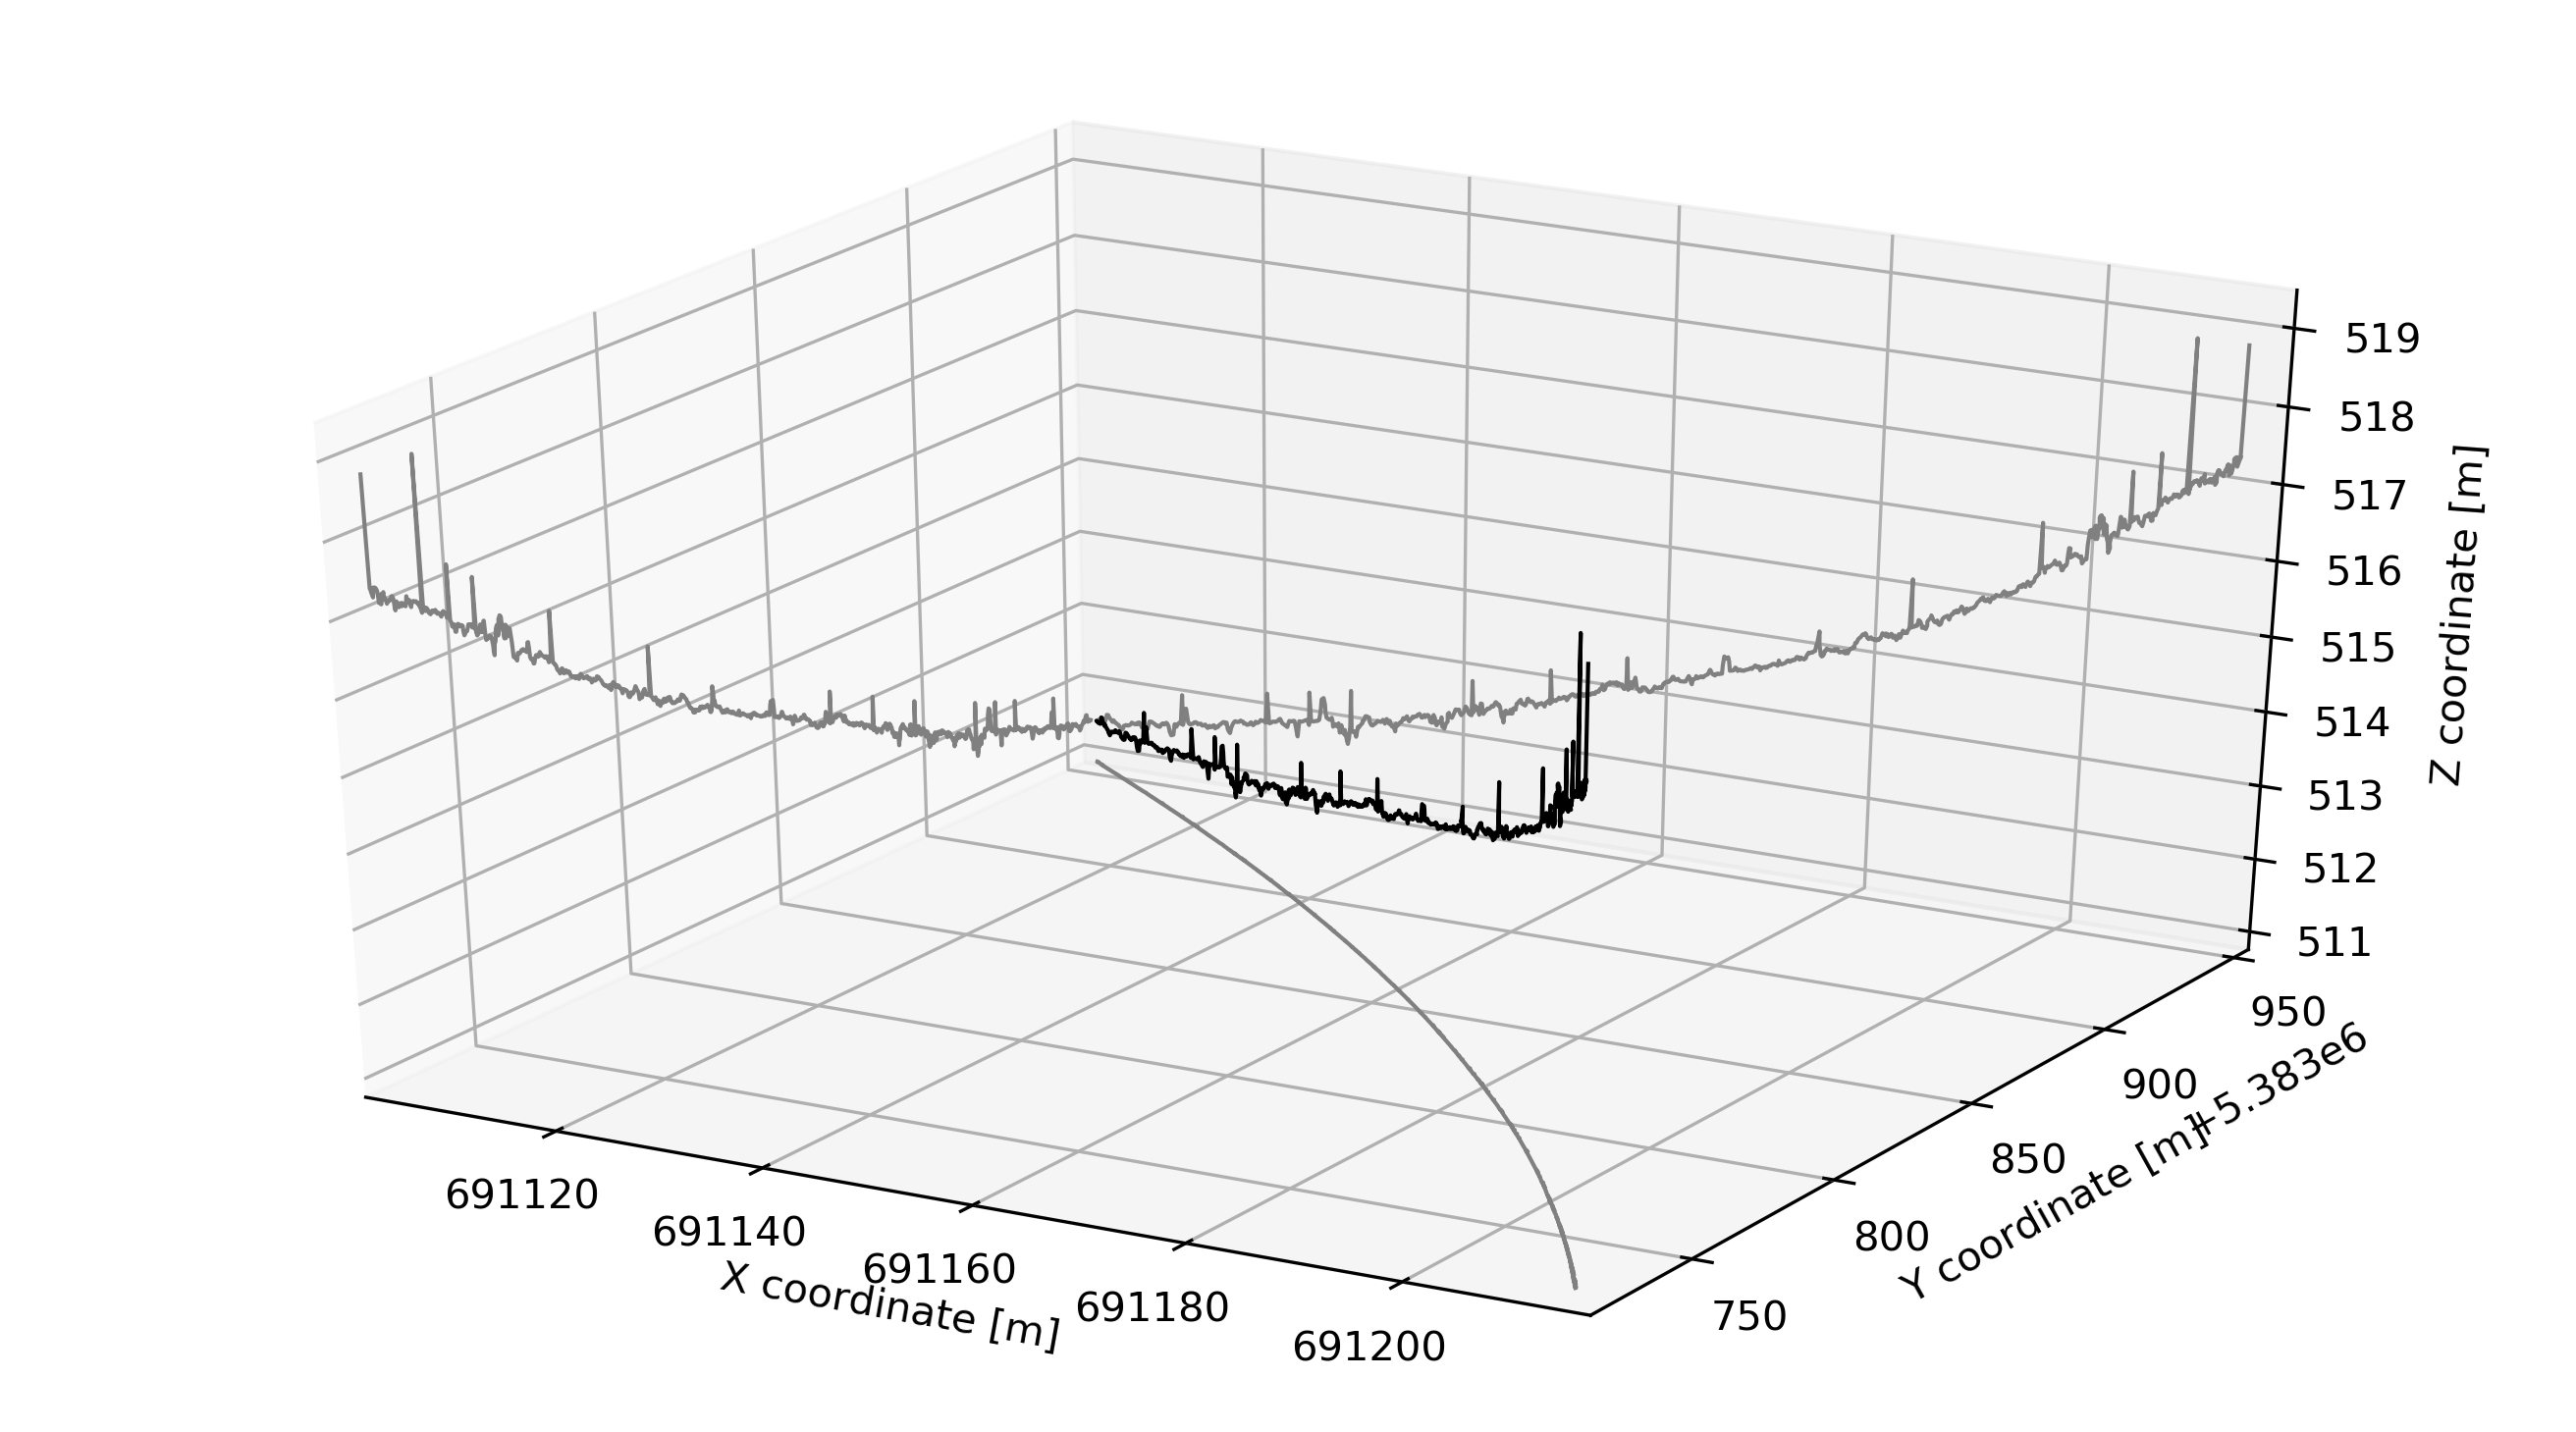
\includegraphics[width=\textwidth]{Test_3D_DSM.png}
	\caption{\small The projected line on DSM.}
	\label{fig:DSMprofile}
\end{figure}


Given image coordinates $\mathbf{p}(x,y)$ of a point and (bundle-adjusted) image orientations $\mathbf{q}$, there is still one degree of freedom in extended collinearity equation \eqref{eq:Gfunction} on solving object coordinates $\mathbf{P}(X,Y,Z)$. Combined with the usage of a DSM, which provides the height information $Z_{DSM}$ given a position $(X,Y)$, the corresponding object coordinates can be solved iteratively until the increment $\Delta Z$ is small enough, i.e. convergence achieved. The iterative scheme is illustrated in \cref{fig:ProjectiononDSM} and \cref{alg:LineProjectionOnDSM}.

Considering that the DSM is raster (discrete) whereas $X$ and $Y$ have continuous numerical values, the DSM height $Z_{DSM}$ for the given point $(X,Y)$ is bilinear interpolated.

\begin{figure}%[!h]
	\centering
	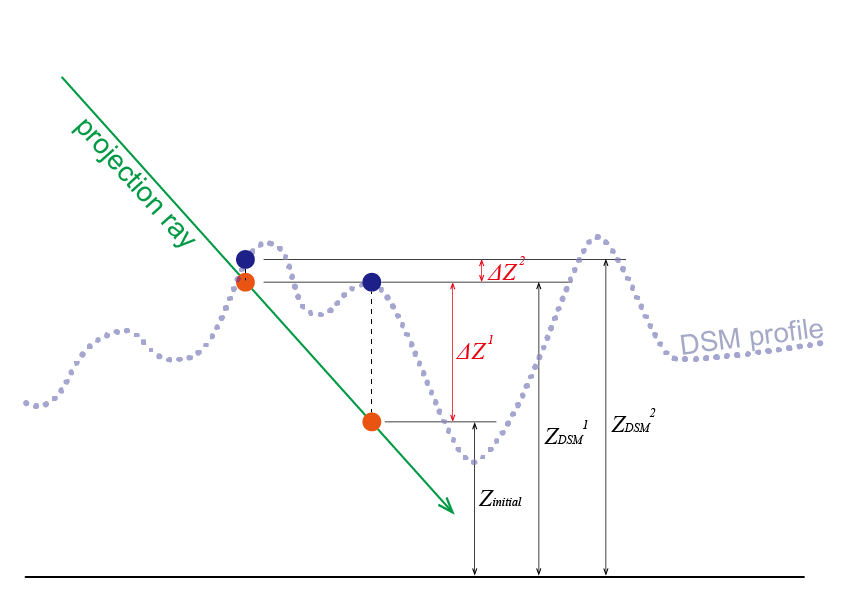
\includegraphics[width=\textwidth]{ProjectionOnDSM.png}
	\caption{\small Iterative scheme of single projection ray intersecting DSM.}
	\label{fig:ProjectiononDSM}
\end{figure}

\begin{Algorithmus}
\caption{Single Point Projection on DSM\newline
	[$X$,$Y$,$Z_{DSM}$]=\texttt{PointProjectionOnDSM}($p(x,y)$,$\mathbf{q}$,$DSM$)\newline
	\textbf{Input}: image coordinates of a point $p(x,y)$, 
					camera parameters $\mathbf{q}$ and
					surface model $DSM$\newline
	\textbf{Output}: object coordinates of the projected point $P(X,Y,Z_{DSM})$ on DSM
}
\label{alg:LineProjectionOnDSM}
\begin{algorithmic}
\State $\Theta=0.5$
\Comment unit: [meter], the convergence threshold
\State $Z_{initial}=500$
\Comment unit: [meter], an initial height value
\State $\Delta Z=9999$
\Comment unit: [meter], an infinite large value approximation
\While{$\Delta Z>\Theta$}
	\State ($X$,$Y$) =$\mathbf{q}$.img2geo($p(x,y)$,$Z_{initial}$)
	\State $Z_{DSM}$ = $DSM$.GetHeight($X$,$Y$)
	\State $\Delta Z=|Z_{DSM}-Z_{initial}|$
	\State $Z_{initial}=Z_{DSM}$
\EndWhile
\State return ($X$,$Y$,$Z_{DSM}$)

\end{algorithmic}
\end{Algorithmus}

